\chapter{MỞ ĐẦU}
\section{KHÁI QUÁT VỀ MÔN VẬT LÍ - VẤN ĐỀ AN TOÀN TRONG VẬT LÍ}
\subsection{LÝ THUYẾT TRỌNG TÂM}
\begin{tomtat}
	\subsubsection{ĐỐI TƯỢNG - MỤC TIÊU - PHƯƠNG PHÁP NGHIÊN CỨU VẬT LÍ}
	\paragraph{Đối tượng nghiên cứu của Vật lí}
	Đối tượng nghiên cứu của Vật lí gồm: các dạng vận động của \textbf{VẬT CHẤT} và \textbf{NĂNG LƯỢNG}.
	\paragraph{Mục tiêu nghiên cứu Vật lí}
	Mục tiêu của vật lí là khám phá ra quy luật tổng quát nhất chi phối sự vận động của vật chất và năng lượng cũng như tương tác giữa chúng ở mọi cấp độ: vi mô, vĩ mô.
	\paragraph{Phương pháp nghiên cứu Vật lí}
	\begin{dn}
		Chất điểm là 
	\end{dn}
	\begin{dl}
		Định luật II Newton
	\end{dl}
	\begin{tc}
		Đặc điểm đường sức từ
	\end{tc}
	\begin{noidung}{Quy tắc nắm tay phải}
		Nắm bàn tay phải
	\end{noidung}
	\begin{luuy}
		Tốc độ dao động khác tốc độ truyền sóng
	\end{luuy}
	\begin{dn}
		\textbf{\textit{Phương pháp thực nghiệm:}} dùng thí nghiệm để phát hiện kết quả mới giúp kiểm chứng, hoàn thiện, bổ sung hay bác bỏ giả thuyết nào đó. Kết quả mới này cần được giải thích bằng lí thuyết đã biết hoặc lí thuyết mới.
	\end{dn}
	\begin{dn}
		\textbf{\textit{Phương pháp lí thuyết:}} sử dụng ngôn ngữ toán học và suy luận lí thuyết để phát hiện một kết quả mới. Kết quả mới này cần được kiểm chứng bằng thực nghiệm.
	\end{dn}
	\begin{note}
		Hai phương pháp hỗ trợ cho nhau, trong đó phương pháp thực nghiệm có tính quyết định.
	\end{note}
	\paragraph{Quy trình tìm hiểu tự nhiên dưới góc độ Vật lí}
	\begin{center}
		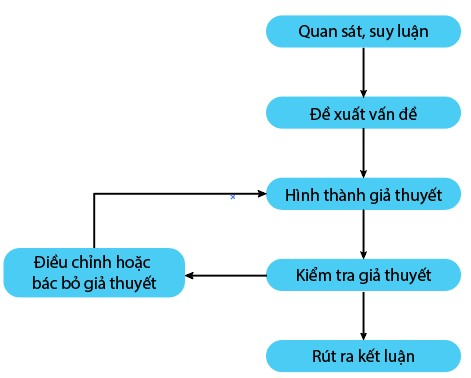
\includegraphics[scale=0.7]{figs/G10Y25B1-2}
	\end{center}
	\subsubsection{Quá trình phát triển của vật lí}
	\begin{center}
		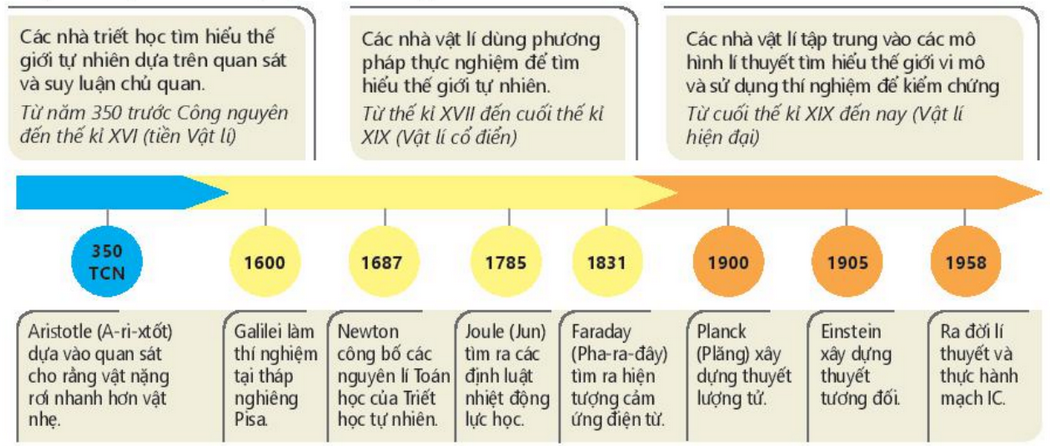
\includegraphics[scale=0.9]{figs/G10Y25B1-1}
	\end{center}
	\subsubsection{Vai trò của vật lí đối với khoa học, kĩ thuật và công nghệ}
	\paragraph{Thông tin liên lạc}
	Khoảng cách địa lí không còn là vấn đề quá lớn của con người trong thông tin liên lạc, sự bùng nổ của mạng lưới internet kết hợp sự phát triển vượt bậc của điện thoại thông minh (smartphone) giúp con người có thể chia sẻ thông tin liên lạc (hình ảnh, giọng nói, tin tức...) một cách dễ dàng.
	\paragraph{Y tế}
	Hầu hết các phương pháp chuẩn đoán và chữa bệnh trong y học đều có cơ sở từ những kiến thức Vật Lý như: chụp X – quang, chụp cộng hưởng từ (MRI), siêu âm, nội soi, xạ trị, \dots
	\paragraph{Công nghiệp}
	Cuộc cách mạng công nghiệp lần thứ tư được coi là bắt đầu thế kỉ XXI. Các nền sản xuất thủ công nhỏ lẻ được thay thế bởi những dây chuyền sản xuất tự động hóa, sử dụng trí tuệ nhân tạo, công nghệ vật liệu (nano), điện toán đám mây.
	\paragraph{Nông nghiệp}
	Việc ứng dụng những thành tựu của Vật Lý vào nông nghiệp đã giúp cho người nông dân tiếp cận với nhiều phương pháp mới, ít tốn lao động, cho năng suất cao. 
	\paragraph{Nghiên cứu khoa học}
	Vật lý góp phần to lớn trong việc cải tiến các thiết bị nghiên cứu khoa học ở nhiều ngành khác nhau như: kính hiển vi điện tử, nhiễu xạ tia X, máy quang phổ, \dots
\end{tomtat}
\subsubsection{Vấn đề an toàn trong Vật lí}
\paragraph{An toàn khi làm việc với phóng xạ}
\begin{enumerate}[label=\arabic*)]
	\item Giữ khoảng cách đủ xa đối với nguồn phóng xạ.
	\item Sử dụng các tấm chắn nguồn phóng xạ đủ tốt.
	\item Giảm thiểu thời gian phơi nhiễm phóng xạ.
\end{enumerate}
\begin{center}
	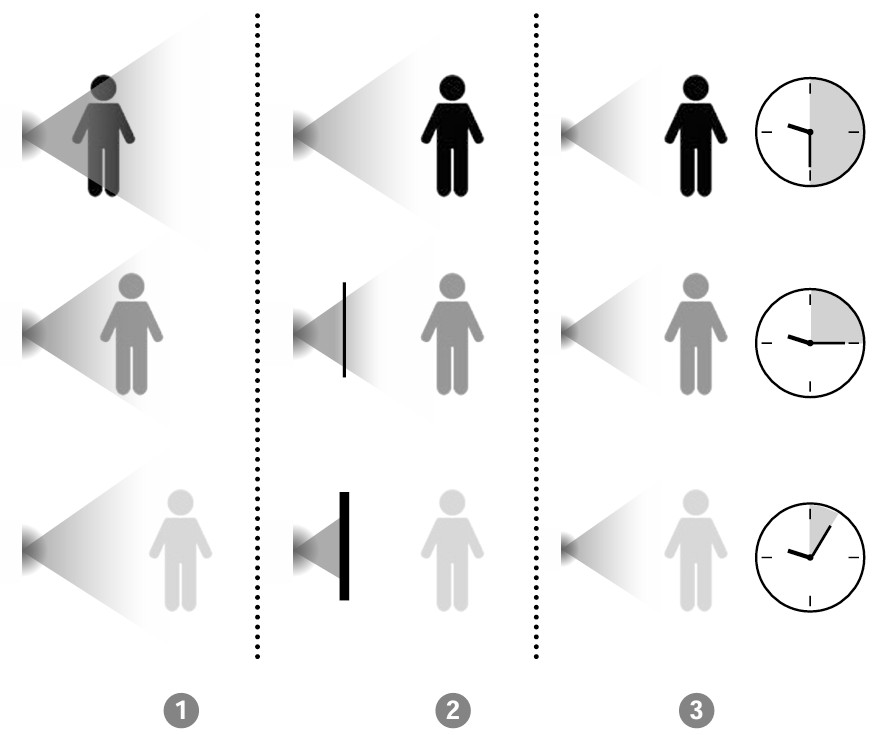
\includegraphics[scale=0.6]{figs/G10Y25B1-3}
\end{center}
\subsubsection{An toàn trong phòng thí nghiệm}
\begin{enumerate}[label=\alph*)]
	\item Một số biện pháp an toàn khi sử dụng điện:
	\begin{itemize}
		\item Trang bị đầy đủ các thiết bị bảo hộ cá nhân.
		\item Giữ khoảng cách an toàn với nguồn điện.
		\item Tránh sử dụng các thiết bị điện khi đang sạc.
		\item Không dùng tay ướt hoặc nhiều mồ hôi khi sử dụng dây điện.
		\item Tránh xa nơi điện thế nguy hiểm.
		\item Lắp đặt vị trí cầu dao, cầu chì, công tắc, ổ điện đúng quy định, \dots
	\end{itemize}
	\item  Khi nghiên cứu và học tập Vật lí cần phải:
	\begin{itemize}
		\item Hiểu được thông tin liên quan đến các rủi ro và nguy hiểm có thể xảy ra.
		\item Tuân thủ và áp dụng các biện pháp bảo vệ để đảm bảo an toàn cho bản thân và cộng đồng.
		\item Quan tâm, gìn giữ và bảo vệ môi trường.
		\item Trong phòng thí nghiệm ở trường học, những rủi ro và nguy hiểm phải được cảnh báo rõ ràng bằng các biển báo. Học sinh cần chú ý sự nhắc nhở của nhân viên phòng thí nghiệm và giáo viên về các quy định an toàn. Ngoài ra, các thiết bị bảo hộ cá nhân cần phải được trang bị đầy đủ.
	\end{itemize}
\end{enumerate}
\subsection{VÍ DỤ MINH HỌA}
\begin{dang}{Phân tích phương trình chuyển động}
	$$x=x_0+vt.$$
	\end{dang}
	% ===================================================================
	\begin{vd}
		
		\choice
		{}
		{}
		{}
		{}
		\loigiai{}
	\end{vd}
\begin{dang}{Nêu được ví dụ về các phương pháp nghiên cứu vật lí}
\end{dang}
\begin{vd}
	Vào đầu thế kỉ XX, J.J.Thomson đã đề xuất mô hình cấu tạo nguyên tử gồm các electron phân bố đều trong một khối điện dương kết cấu tựa như khối mây. Để kiểm chứng giả thuyết này, E. Rutherford đã sử dụng tia alpha gồm các hạt mang điện dương bắn vào các nguyên tử kim loại vàng Hình \ref{fig:2.2}. Kết quả của thí nghiệm đã bác bỏ giả thuyết của J. J. Thomson, đồng thời đã giúp khám phá ra hạt nhân nguyên tử. E. Rutherford đã vận dụng phương pháp nghiên cứu nào để nghiên cứu vấn đề này? Giải thích.
	\begin{center}
		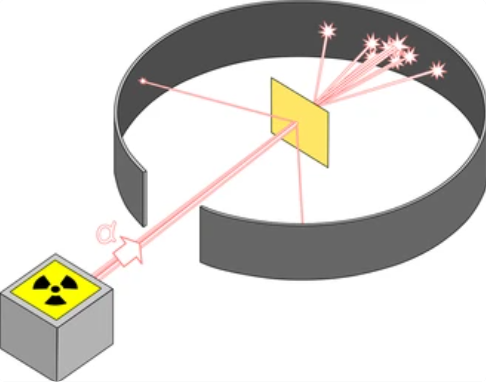
\includegraphics[scale=0.3]{figs/G10Y25B1-4}
		\captionof{figure}{Thí nghiệm Rutherford.}
		\label{fig:2.2}
	\end{center}
	\loigiai{
		Rutherford đã sử dụng phương pháp thực nghiệm trong nghiên cứu vật lí vì ông đã thực hiện thí nghiệm dùng tia alpha gồm các hạt mang điện dương bắn vào các nguyên tử vàng để phát hiện ra kết quả mới chính là hạt nhân nguyên tử.
	}
\end{vd}
\begin{dang}{Mô tả được các bước \\trong tiến trình tìm hiểu thế giới tự nhiên}
\end{dang}
\begin{vd}
	Sắp xếp các bước tiến hành quá trình tìm hiểu thế giới tự nhiên dưới góc độ vật lí:
	\begin{enumerate}[label= (\arabic*)]
		\item Phân tích số liệu.
		\item Quan sát, xác định đối tượng cần nghiên cứu.
		\item Thiết kế, xây dựng mô hình kiểm chứng giả thuyết.
		\item Đề xuất giả thuyết nghiên cứu.
		\item Rút ra kết luận.
	\end{enumerate}
	\loigiai{
		Tiến trình tìm hiểu thế giới tự nhiên dưới góc độ Vật lí là (2) - (4) - (3) - (1) - (5).
	}
\end{vd}
\begin{dang}{Vấn đề an toàn trong Vật lí}
\end{dang}
\begin{vd}
	Trạm không gian quốc tế ISS có độ cao khoảng \SI{400}{km}, trong khi bầu khí quyển có bề dày hơn \SI{100}{km}. Trong trạm không gian có tình trạng mất trọng lượng, mọi vật sẽ tự do lơ lửng. Hãy tìm hiểu các bất thường và nguy hiểm mà các nhà du hành làm việc lâu dài ở trong trạm có thể gặp phải.
	\loigiai{
	\begin{itemize}
		\item Không có tầng ozone bảo vệ, các phi hành gia dễ bị tia cực tím gây hại gây các bệnh về da.
		\item Mọi vật đều lơ lửng nên khó khăn trong sinh hoạt.
		\item Nguy hiểm từ các mảnh thiên thạch trôi nổi trong không gian.
		\item Ảnh hưởng sinh lí do sống lâu trong không gian.
	\end{itemize}
	}
	
\end{vd}

\subsection{TRẮC NGHIỆM NHIỀU PHƯƠNG ÁN LỰA CHỌN}
\setcounter{ex}{0}
\Opensolutionfile{ans}[ans/G10Y25B1-TN]
\begin{ex}
	Đối tượng nghiên cứu của Vật lí là gì?
	\choice
	{Các dạng vận động và tương tác của vật chất}
	{Quy luật tương tác của các dạng năng lượng}
	{\True Các dạng vận động của vật chất và năng lượng}
	{Quy luật vận động, phát triển của sự vật - hiện tượng}
	\loigiai{}
\end{ex}

\begin{ex}
	Lĩnh vực nghiên cứu nào sau đây là của Vật lí?
	\choice
	{Nghiên cứu về sự thay đổi của các chất khi kết hợp với nhau}
	{Nghiên cứu sự phát triển của vi khuẩn}
	{Nghiên cứu về sự hình thành và phát triển của các tầng lớp, giai cấp trong xã hội}
	{\True Nghiên cứu về các dạng chuyển động và các dạng năng lượng khác nhau}
	\loigiai{}
\end{ex}

\begin{ex}
	Cách sắp xếp nào sau đây trong 5 bước của phương pháp thực nghiệm là đúng?
	\choice
	{Xác định vấn đề cần nghiên cứu, dự đoán, quan sát, thí nghiệm, kết luận}
	{Quan sát, xác định vấn đề cần nghiên cứu, thí nghiệm, dự đoán, kết luận}
	{\True Xác định vấn đề cần nghiên cứu, quan sát, dự đoán, thí nghiệm, kết luận}
	{Thí nghiệm, xác định vấn đề cần nghiên cứu, dự đoán, quan sát, kết luận}
	\loigiai{}
\end{ex}

\begin{ex}
	Thành tựu nghiên cứu nào sau đây của Vật lí được coi là có vai trò quan trọng trong việc mở đầu cho cuộc cách mạng công nghệ lần thứ nhất?
	\choice
	{Nghiên cứu về lực vạn vật hấp dẫn}
	{\True Nghiên cứu về nhiệt động lực học}
	{Nghiên cứu về cảm ứng điện từ}
	{Nghiên cứu về thuyết tương đối}
	\loigiai{}
\end{ex}

\begin{ex}
	Từ việc quan sát sự rơi của các vật nặng nhẹ khác nhau mà Aristotle, một nhà khoa học Hy Lạp sống vào những năm 300 trước Công nguyên cho rằng: "Vật nặng rơi nhanh hơn vật nhẹ, vật càng nặng rơi càng nhanh". Yếu tố nào sau đây là quan trọng nhất dẫn tới việc Aristotle mắc sai lầm khi xác định nguyên nhân làm cho các vật rơi nhanh chậm khác nhau?
	\choice
	{Khoa học chưa phát triển}
	{Ông quá tự tin vào suy luận của mình}
	{Không có nhà khoa học nào khác giúp đỡ ông}
	{\True Ông không làm thí nghiệm để kiểm tra quan điểm của mình}
	\loigiai{}
\end{ex}

\begin{ex}
	Đối tượng nghiên cứu của vật lí là gì?
	\choice
	{Các dạng vận động và tương tác của vật chất}
	{Quy luật tương tác của các dạng năng lượng}
	{\True Các dạng vận động của vật chất và năng lượng}
	{Quy luật vận động, phát triển của sự vật hiện tượng}
	\loigiai{}
\end{ex}
<<<<<<< Updated upstream
\Closesolutionfile{ans}
\subsection{TRẮC NGHIỆM ĐÚNG SAI}
\setcounter{ex}{0}
\Opensolutionfile{ans}[ans/G10Y25B1-TF]
% ===================================================================
\begin{ex}
	
	\choiceTF[t]
	{}
	{}
	{}
	{}
	\loigiai{}
\end{ex}
\Closesolutionfile{ans}
\subsection{TỰ LUẬN}
\setcounter{ex}{0}
\Opensolutionfile{ans}[ans/G10Y25B1-TL]

\Closesolutionfile{ans}
=======

\begin{ex}
	Mục tiêu của môn Vật lí là
	\choice
	{\True khám phá ra quy luật tổng quát nhất chi phối sự vận động của vật chất và năng lượng, cũng như tương tác giữa chúng ở mọi cấp độ: vi mô, vĩ mô}
	{khám phá ra quy luật tổng quát nhất chi phối sự vận động của vật chất và năng lượng}
	{khảo sát sự tương tác của vật chất ở mọi cấp độ: vi mô, vĩ mô}
	{khám phá ra quy luật vận động cũng như tương tác của vật chất ở mọi cấp độ: vi mô, vĩ mô}
	\loigiai{}
\end{ex}

\begin{ex}
	Cấp độ vi mô là
	\choice
	{\True cấp độ dùng để mô phỏng vật chất nhỏ bé}
	{cấp độ to, nhỏ tùy thuộc vào quy mô được khảo sát}
	{cấp độ dùng để mô phỏng tầm rộng lớn hay rất lớn của vật chất}
	{cấp độ tinh vi khi khảo sát một hiện tượng vật lí}
	\loigiai{}
\end{ex}

\begin{ex}
	Cấp độ vĩ mô là
	\choice
	{cấp độ dùng để mô phỏng vật chất nhỏ bé}
	{cấp độ to, nhỏ tùy thuộc vào quy mô được khảo sát}
	{\True cấp độ dùng để mô phỏng tầm rộng lớn hay rất lớn của vật chất}
	{cấp độ tinh vi khi khảo sát một hiện tượng vật lí}
	\loigiai{}
\end{ex}

\begin{ex}
	Chọn câu đúng khi nói về phương pháp thực nghiệm.
	\choice
	{Hai phương pháp thực nghiệm và lí thuyết hỗ trợ cho nhau, trong đó phương pháp lí thuyết có tính quyết định}
	{Phương pháp thực nghiệm sử dụng ngôn ngữ toán học và suy luận lí thuyết để phát hiện một kết quả mới}
	{\True Phương pháp thực nghiệm dùng thí nghiệm để phát hiện kết quả mới giúp kiểm chứng, hoàn thiện, bổ sung hay bác bỏ giả thuyết nào đó}
	{Kết quả được phát hiện từ phương pháp thực nghiệm cần được kiểm chứng bằng lí thuyết}
	\loigiai{}
\end{ex}

\begin{ex}
	Kết luận đúng về ảnh hưởng của vật lí đến một số lĩnh vực trong đời sống và kĩ thuật.
	\choice
	{Vật lí là cơ sở của khoa học tự nhiên và công nghệ}
	{Vật lí ảnh hưởng đến một số lĩnh vực: Thông tin liên lạc; Y tế; Công nghiệp; Nông nghiệp; Nghiên cứu khoa học}
	{Dựa trên nền tảng vật lí các công nghệ mới được sáng tạo với tốc độ vũ bão}
	{\True Tất cả đều đúng}
	\loigiai{}
\end{ex}

\begin{ex}
	Hiện tượng vật lí nào sau đây liên quan đến phương pháp thực nghiệm?
	\choice
	{Ô tô khi chạy đường dài có thể xem ô tô như là một chất điểm}
	{\True Thả rơi một vật từ trên cao xuống mặt đất}
	{Quả địa cầu là mô hình thu nhỏ của Trái đất}
	{Để biểu diễn đường truyền của ánh sáng người ta dùng tia sáng}
	\loigiai{}
\end{ex}

\begin{ex}
	Hiện tượng vật lí nào sau đây liên quan đến phương pháp lí thuyết?
	\choice
	{\True Ô tô khi chạy đường dài có thể xem ô tô như là một chất điểm}
	{Thả rơi một vật từ trên cao xuống mặt đất}
	{Kiểm tra sự thay đổi nhiệt độ trong quá trình nóng chảy hoặc bay hơi của một chất}
	{Ném một quả bóng lên trên cao}
	\loigiai{}
\end{ex}

\begin{ex}
	Những ngành nghiên cứu nào thuộc về vật lí
	\choice
	{\True Cơ học, nhiệt học, điện học và quang học}
	{Nhiệt học, quang học và sinh vật học}
	{Điện học, quang học và xã hội học}
	{Cơ học, nhiệt học và địa lý học}
	\loigiai{}
\end{ex}

\begin{ex}
	Ai được mệnh danh là “cha đẻ” của phương pháp thực nghiệm
	\choice
	{Isaac Newton}
	{\True Galileo Galilei}
	{Albert Einstein}
	{James Watt}
	\loigiai{}
\end{ex}

\begin{ex}
	Thành tựu nghiên cứu nào sau đây của Vật lí được coi là có vai trò quan trọng trong việc mở đầu cho cuộc cách mạng công nghiệp lần thứ hai vào cuối thế kỉ XIX?
	\choice
	{Nghiên cứu về lực vạn vật hấp dẫn}
	{Nghiên cứu về nhiệt động lực học}
	{\True Nghiên cứu về cảm ứng điện từ}
	{Nghiên cứu về thuyết tương đối}
	\loigiai{}
\end{ex}

\begin{ex}
	Đặc trưng cơ bản của cuộc cách mạng công nghiệp lần thứ ba ở thế kỉ XX là
	\choice
	{\True tự động hóa các quá trình sản xuất}
	{sự xuất hiện các thiết bị dùng điện trong mọi lĩnh vực sản xuất và đời sống con người}
	{thay thế sức lực cơ bắp bằng sức lực máy móc}
	{sử dụng trí tuệ nhân tạo, robot, internet toàn cầu, công nghệ vật liệu nano}
	\loigiai{}
\end{ex}

\begin{ex}
	Đặc trưng của cuộc cách mạng công nghiệp lần thứ tư vào đầu thế kỉ XXI là
	\choice
	{Xây dựng các dây chuyển sản suất tự động dựa trên những thành tựu nghiên cứu về điện tử,vi mạch, chất bán dẫn, ...}
	{\True Sử dụng trí tuệ nhân tạo, robot, internet toàn cầu, công nghệ vật liệu siêu nhỏ, điện thoại thông minh, ...}
	{Xuất hiện các thiết bị dùng điện trong mọi lĩnh vực sản xuất và đời sống con người}
	{Thay thế sức lực cơ bắp bằng sức lực máy móc}
	\loigiai{}
\end{ex}

\begin{ex}
	Chọn phát biểu chính xác nhất? Dự đoán khoa học là một dự đoán có cơ sở dựa trên yếu tố
	\choice
	{suy luận từ những hiện tượng khác có tính tương đồng}
	{quan sát, trải nghiệm thực tế}
	{\True quan sát, trải nghiệm thực tế, các kiến thức đã có liên quan đến dự đoán}
	{suy luận từ những thí nghiệm liên quan đến hiện tượng khác}
	\loigiai{}
\end{ex}

\begin{ex}
	Sau khi đưa ra một dự đoán khoa học thì người ta phải
	\choice
	{kết luận}
	{\True làm thí nghiệm để kiểm tra}
	{xác định vấn đề nghiên cứu}
	{tiếp tục đưa ra dự đoán mới}
	\loigiai{}
\end{ex}

\begin{ex}
	Khi nói về những quy tắc an toàn khi làm việc với phóng xạ, phát biểu nào sau đây là \textbf{sai}?
	\choice
	{Giảm thời gian tiếp xúc với nguồn phóng xạ}
	{Tăng khoảng cách từ ta đến nguồn phóng xạ}
	{Đảm bảo che chắn những cơ quan trọng yếu của cơ thể}
	{\True Mang áo phòng hộ và không cần đeo mặt nạ}
	\loigiai{}
\end{ex}

\begin{ex}
	Kí hiệu “Input (I)” mang ý nghĩa là
	\choice
	{cực dương}
	{cực âm}
	{\True đầu vào}
	{đầu ra}
	\loigiai{}
\end{ex}

\begin{ex}
	Chọn đáp án \textbf{sai}? Cần tuân thủ các biển báo an toàn trong phòng thực hành nhằm mục đích
	\choice
	{\True tạo ra nhiều sản phẩm mang lại lợi nhuận}
	{hạn chế các trường hợp nguy hiểm như: đứt tay, ngộ độc,…}
	{tránh được các tổn thất về tài sản nếu không làm theo hướng dẫn}
	{phòng chống cháy, nổ}
	\loigiai{}
\end{ex}

\begin{ex}
	Biển báo \vspace{-0.5cm}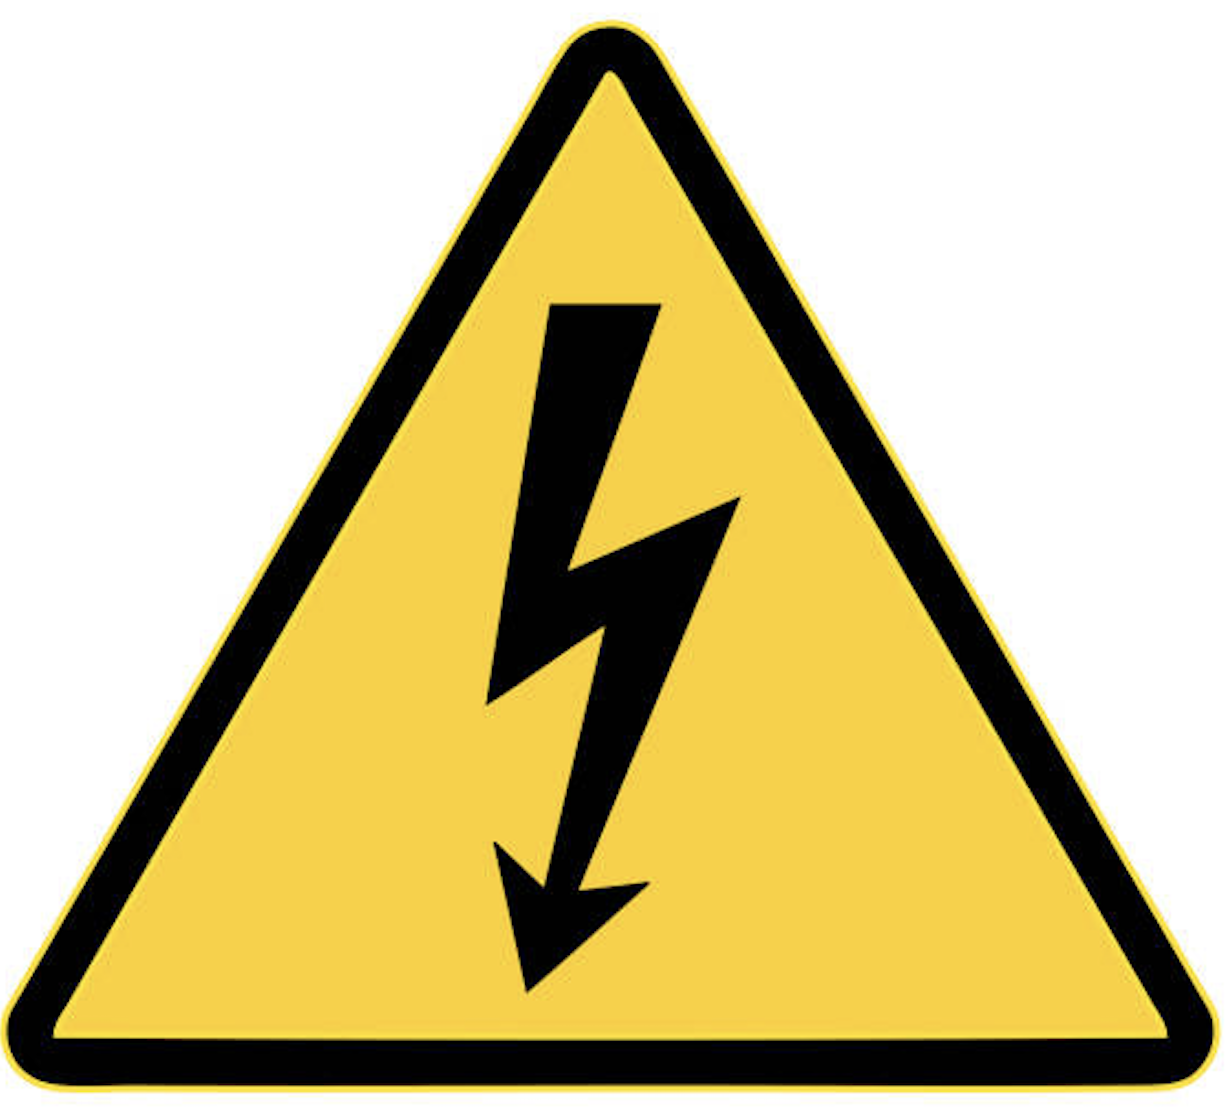
\includegraphics[scale=0.1]{figs/G10Y25B1-5} mang ý nghĩa gì?\\
	\choice
	{\True Nơi nguy hiểm về điện}
	{Lưu ý cẩn thận}
	{Cẩn thận sét đánh}
	{Cảnh báo tia laser}
	\loigiai{}
\end{ex}

\begin{ex}
	Biển báo \vspace{-0.5cm}
\includegraphics[scale=0.2]{figs/G10Y25B1-6} mang ý nghĩa gì?\\
	\choice
	{Nơi cấm sử dụng quạt}
	{Tránh gió trực tiếp}
	{Lối thoát hiểm}
	{\True Nơi có chất phóng xạ}
	\loigiai{}
\end{ex}

\begin{ex}
	Chọn đáp án sai khi nói về những quy tắc an toàn trong phòng thí nghiệm.
	\choice
	{Đọc kĩ hướng dẫn sử dụng thiết bị và quan sát các chỉ dẫn, các kí hiệu trên các thiết bị thí nghiệm}
	{\True Tắt công tắc nguồn thiết bị điện sau khi cắm hoặc tháo thiết bị điện}
	{Kiểm tra cẩn thận thiết bị, phương tiện, dụng cụ thí nghiệm trước khi sử dụng}
	{Chỉ tiến hành thí nghiệm khi được sự cho phép của giáo viên hướng dẫn thí nghiệm}
	\loigiai{}
\end{ex}

\begin{ex}
	Chọn đáp án đúng khi nói về những quy tắc an toàn trong phòng thí nghiệm.
	\choice
	{Tắt công tắc nguồn thiết bị điện sau khi cắm hoặc tháo thiết bị điện}
	{Tuyệt đối không tiếp xúc với các vật và các thiết bị thí nghiệm có nhiệt độ cao ngay khi có dụng cụ bảo hộ}
	{Được phép tiến hành thí nghiệm khi đã mang đồ bảo hộ}
	{\True Phải vệ sinh, sắp xếp gọn gàng, các thiết bị và dụng cụ thí nghiệm, bỏ chất thải thí nghiệm vào đúng nơi quy định sau khi tiến hành thí nghiệm}
	\loigiai{}
\end{ex}

\begin{ex}
	Khi gặp sự cố mất an toàn trong phòng thực hành, học sinh cần
	\choice
	{\True báo cáo ngay với giáo viên trong phòng thực hành}
	{tự xử lí và không báo với giáo viên}
	{nhờ bạn xử lí sự cố}
	{tiếp tục làm thí nghiệm}
	\loigiai{}
\end{ex}

\begin{ex}
	Khi phòng thực hành xuất hiện cháy thì ta cần phải
	\choice
	{chạy ra khỏi phòng, đi tìm thêm người đến dập đám cháy}
	{\True ngắt điện, di chuyển các chất dễ cháy ra ngoài và chống cháy lan, cứu người, cứu tài sản, dập tắt đám cháy}
	{ngắt nguồn điện, dùng nước dập đám cháy}
	{dùng nước dập đám cháy}
	\loigiai{}
\end{ex}

\begin{ex}
	Trong bài thực hành có sử dụng mạch điện nhưng khi lắp ráp xong mạch điện, báo cáo giáo viên phụ trách rồi cắm vào nguồn điện nhưng mạch không vào điện thì học sinh cần
	\choice
	{kiểm tra lại mạch điện}
	{kiểm tra nguồn điện}
	{ngắt mạch điện ra khỏi nguồn}
	{\True ngắt mạch điện ra khỏi nguồn sau đó kiểm tra mạch điện và nguồn điện}
	\loigiai{}
\end{ex}

\subsection{TRẮC NGHIỆM ĐÚNG SAI}
\setcounter{ex}{0}
\begin{ex}
	Đối tượng nghiên cứu và mục tiêu của Vật lí:
	\choiceTF[t]
	{\True Đối tượng nghiên cứu của Vật lí gồm: các dạng vận động của vật chất và năng lượng}
	{\True Mục tiêu của Vật lí là khám phá ra quy luật tổng quát nhất chi phối sự vận động của vật chất và năng lượng, cũng như tương tác giữa chúng ở mọi cấp độ vi mô và vĩ mô}
	{Mục tiêu học tập môn Vật lí: Giúp học sinh hình thành, phát triển năng lực Toán học}
	{Cấp độ vĩ mô là là cấp độ dùng để mô phỏng vật chất nhỏ bé}
	\loigiai{\begin{itemchoice}
			\itemch Đúng.
			\itemch Đúng.
			\itemch Sai. Mục tiêu học tập môn Vật lí: Giúp học sinh hình thành, phát triển năng lực vật lí.
			\itemch Sai. Cấp độ vĩ mô là cấp độ dùng để mô phỏng tầm rộng lớn hay rất lớn của vật chất.
	\end{itemchoice}}
\end{ex}
\begin{ex}
	Quá trình phát triển của Vật lí trải qua 3 giai đoạn.
	\choiceTF[t]
	{\True Giai đoạn 1: Các nhà triết học tìm hiểu thế giới tự nhiên dựa trên quan sát và suy luận chủ quan: từ năm 350 trước Công nguyên đến thế kỉ XVI (tiền Vật lí)}
	{\True Giai đoạn 2: Các nhà vật lý dùng phương pháp thực nghiệm để tìm hiểu thế giới tự nhiên: từ thế kỉ XVII đến cuối thế kỉ XIX (Vật lí cổ điển)}
	{Giai đoạn 3: Các nhà vật lý tập trung vào các mô hình thực nghiệm tìm hiểu thế giới vĩ mô: Từ cuối thế kỉ XIX đến nay (Vật lí hiện đại)}
	{Việc ứng dụng các thành tựu của vật lý vào công nghệ luôn mang lại lợi ích cho nhân loại, không có tác hại gì}
	\loigiai{\begin{itemchoice}
			\itemch Đúng.
			\itemch Đúng.
			\itemch Sai. Giai đoạn 3: Các nhà vật lý tập trung vào các mô hình lí thuyết tìm hiểu thế giới \textbf{vi mô} và sử dụng thí nghiệm để kiểm chứng: Từ cuối thế kỉ XIX đến nay (Vật lí hiện đại).
			\itemch Sai. Việc ứng dụng các thành tựu của vật lý vào công nghệ không chỉ mang lại lợi ích cho nhân loại mà còn có thể làm ô nhiễm môi trường sống, hủy hoại hệ sinh thái,… nếu không được sử dụng đúng phương pháp, đúng mục đích.
	\end{itemchoice}}
\end{ex}
\begin{ex}
	Để đảm bảo an toàn trong phòng thí nghiệm, ta cần phải
	\choiceTF[t]
	{\True Nhờ giáo viên kiểm tra mạch điện trước khi bật nguồn điện}
	{Dùng tay ướt cắm điện vào nguồn điện}
	{\True Rửa sạch da khi tiếp xúc với hóa chất}
	{Để các thiết bị nối với nguồn điện giúp duy trì năng lượng}
	\loigiai{\begin{itemchoice}
			\itemch Đúng.
			\itemch Sai. 
			\itemch Đúng.
			\itemch Sai.
	\end{itemchoice}}
\end{ex}
\begin{ex}
	\immini{Hình bên là đồng hồ đa năng hiện số dùng để đo hiệu điện thế, cường độ dòng điện, điện trở,...
	\choiceTF
	{\True Điều chỉnh thang đo trên đồng hồ đa năng bằng cách vặn núm điều chỉnh ở giữa đồng hồ về vị trí cần tìm}
	{Vặn núm quay về bên trái để đo cường độ dòng điện}
	{\True Vặn núm quay về bên trái để đo hiệu điện thế}
	{Kí hiệu AC là dòng điện một chiều, DC là dòng điện xoay chiều}
	}
	{\vspace{-0.5cm}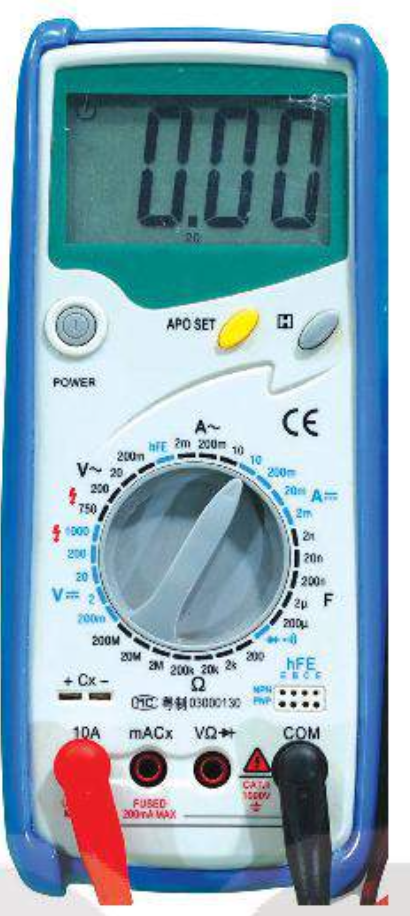
\includegraphics[scale=0.3]{figs/G10Y25B1-7}}
	
	\loigiai{\begin{itemchoice}
			\itemch Đúng.
			\itemch Sai. Vặn núm quay về bên phải.
			\itemch Đúng.
			\itemch Sai. Kí hiệu AC là dòng điện xoay chiều, DC là dòng điện một chiều.
	\end{itemchoice}}
\end{ex}

\subsection{TRẮC NGHIỆM TRẢ LỜI NGẮN}
\setcounter{ex}{0}

\begin{ex} 
	Quá trình phát triển của Vật lí trải qua bao nhiêu giai đoạn chính?
	\shortans[oly]{3}
	\loigiai{Tiền Vật lí, Vật lí cổ điển, Vật lí hiện đại}
\end{ex}
\begin{ex} 
	Lịch sử loài người đã trải qua bao nhiêu cuộc cách mạng công nghiệp dựa trên những kết quả nghiên cứu của Vật lí?
	\shortans[oly]{4}
	\loigiai{}
\end{ex}
\begin{ex} 
	Trong những hoạt động sau, có bao nhiêu hoạt động tuân thủ nguyên tắc an toàn khi làm việc với nguồn phóng xạ?
	\begin{enumerate}[label=\arabic*.]
		\item Sử dụng phương tiện phòng hộ cá nhân như quần áo phòng hộ, mũ, găng tay, áo chì.
		\item Ăn uống, trang điểm trong phòng làm việc có chứa chất phóng xạ.
		\item Tẩy xạ khi bị nhiễm bẩn phóng xạ theo quy định.
		\item Đổ rác thải phóng xạ tại các khu tập trung tác thải sinh hoạt.
		\item Mang nguồn phóng xạ về nhà luyện tập.
	\end{enumerate}
	\shortans[oly]{2}
	\loigiai{Hoạt động 1 và 3.}
\end{ex}
\begin{ex} 
	Có bao nhiêu biển báo mang ý nghĩa cảnh báo nguy hiểm trong hình bên dưới?
	\begin{center}
		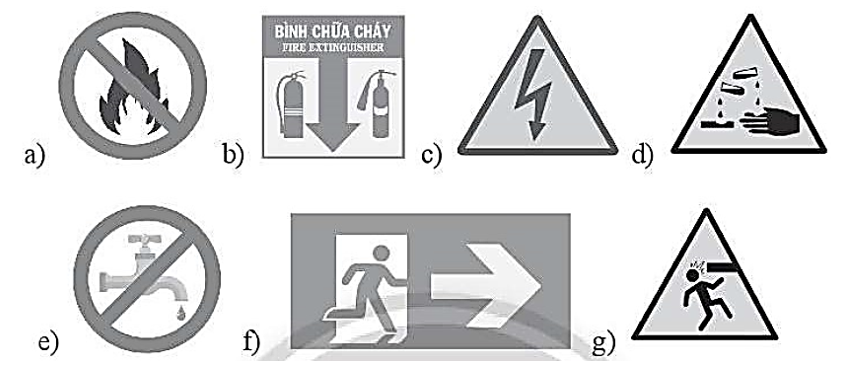
\includegraphics[scale=0.5]{figs/G10Y25B1-8}
	\end{center}
	\shortans[oly]{3}
	\loigiai{c, d và g.}
\end{ex}
\Closesolutionfile{ans}
\subsection{TỰ LUẬN}
\setcounter{ex}{0}
%\Opensolutionfile{ans}[ans/G10Y25B1-TL]
\begin{ex}
	Khi chiếu ánh sáng đến gương, ta quan sát thấy ánh sáng bị gương hắt trở lại môi trường cũ. Thực hiện những khảo sát chi tiết, ta có thể rút ra kết luận về nội dung định luật phản xạ ánh sáng như sau:\\
	-	Khi ánh sáng bị phản xạ, tia phản xạ sẽ nằm trong mặt phẳng chứa tia sáng tới và pháp tuyến của gương tại điểm tới.\\
	-	Góc phản xạ sẽ bằng góc tới.\\
	Hãy xác định đối tượng nghiên cứu và phương pháp nghiên cứu trong khảo sát trên.
	\loigiai{
	Đối tượng nghiên cứu: Sự truyền ánh sáng khi đến mặt gương.\\
	Phương pháp nghiên cứu: Phương pháp thực nghiệm.}
\end{ex}
\begin{ex}
	Cuộc cách mạng khoa học lần thứ nhất được đánh dấu bởi sự kiện khoa học nào? Đặc trưng của cuộc cách mạng khoa học lần thứ nhất là gì?
	\loigiai{
		Sự ra đời của động cơ hơi nước.\\
		Đặc trưng: thay thế sức lực của con người bằng sức lực của máy móc.}
\end{ex}
\begin{ex}
	Trình bày một số ví dụ minh họa cho phương pháp thực nghiệm trong Vật lí.
	\loigiai{
		Thí nghiệm tạo ra âm thanh (như gảy đàn, gõ vào thanh kim loại, ...) để chứng tỏ âm thanh truyền được trong chất rắn, lỏng, khí.\\
		Thí nghiệm sử dụng ánh sáng để đốt cháy tờ giấy, từ đó có thể nêu được ánh sáng có năng lượng.}
\end{ex}
\begin{ex}
	Tìm hiểu thực tế một số thiết bị vật lí dùng trong y tế để chẩn đoán, đo lường và chữa bệnh.
	\loigiai{
		\begin{enumerate}[label=\arabic*)]
			\item Các sợi quang dùng trong nội soi ứng dụng kiến thức về phản xạ toàn phần.
			\item Máy kích tim ứng dụng kiến thức về các tác dụng sinh lí của dòng điện.
			\item Máy chụp X quang.
			\item Máy đo tật khúc xạ của mắt ứng dụng kiến thức về định luật khúc xạ và thấu kính.
		\end{enumerate}
	}
\end{ex}
\begin{ex}
	Trình bày ví dụ chứng tỏ kiến thức Vật lí giúp tránh được nguy cơ tổn hại tài sản.
	\loigiai{
		Kiến thức về điện từ giúp mô tả được cách dòng điện chạy qua các mạch điện trong gia đình, hiểu được các phương pháp bảo vệ mạch điện, tránh được các vụ cháy nổ do chập điện...}
\end{ex}
\begin{ex}
	Ở những nơi nhiệt độ thấp (dưới \SI{0}{\celsius}), người ta nhận thấy rằng khi vung cùng một lượng nước nhất định ra không khí thì nước nóng sẽ đông đặc nhanh hơn so với nước lạnh. Em hãy xây dựng tiến trình tìm hiểu hiện tượng trên.
	\loigiai{
		\begin{enumerate}[label=Bước \arabic*:, leftmargin=2cm]
		\item \textit{Quan sát, suy luận:} “Nước nóng sẽ đông đặc nhanh hơn so với nước lạnh”.
		\item \textit{Đề xuất vấn đề:} Sự ảnh hưởng của nhiệt độ ban đầu đến thời gian đông đặc của nước.
		\item \textit{Hình thành giả thuyết:} Nước nóng sẽ đông đặc nhanh hơn so với nước lạnh.
		\item \textit{Kiểm tra giả thuyết:}\\
			Lập phương án thí nghiệm khảo sát thời gian đông đặc của hai cốc nước có nhiệt độ khác nhau khi cho vào ngăn đông của tủ lạnh.\\
			Tiến hành thí nghiệm. Pha hai cốc nước (cùng thể tích) có nhiệt độ 50C và 350C. Đặt 2 cốc nước và ngăn đông của tủ lạnh. Quan sát trạng thái đông đặc của hai cốc nước sau mỗi một giờ. Thu thập, xử lí và phân tích dữ liệu thực nghiệm.
		\item \textit{Rút ra kết luận}.
		\end{enumerate}
	}
\end{ex}
\begin{ex}
	Trong các hoạt động dưới đây, hoạt động nào dưới đây, hoạt động nào đảm bảo an toàn và những hoạt động nào gây nguy hiểm khi vào phòng thí nghiệm.
	\begin{enumerate}[label=\arabic*.]
		\item Mặc áo blouse, mang bao tay, kính bảo hộ trước khi vào phòng thí nghiệm.
		\item Nhờ giáo viên kiểm tra mạch điện trước khi bật nguồn điện.
		\item Dùng tay ướt cắm điện vào nguồn điện.
		\item Mang đồ ăn, thức uống vào phòng thí nghiệm.
		\item Thực hiện thí nghiệm nhanh và mạnh.
		\item Bỏ chất thải thí nghiệm vào đúng nơi quy định.
		\item Chạy nhảy, vui đùa trong phòng thí nghiệm.
		\item Rửa sạch da khi tiếp xúc với hóa chất.
		\item Tự ý đem đồ thí nghiệm mang về nhà luyện tập.
		\item Buộc tóc gọn gàng, tránh để tóc tiếp xúc với hóa chất và dụng cụ thí nghiệm.
	\end{enumerate}
	\loigiai{
		An toàn: 1, 2, 6, 8, 10.\\
		Nguy hiểm: 3, 4, 5, 7, 9.
	}
\end{ex}
\begin{ex}
	\immini {Trong quá trình thực hành tại phòng thí nghiệm, một bạn học sinh vô tình làm vỡ nhiệt kế thuỷ ngân và làm thuỷ ngân đổ ra ngoài như hình bên. Em hãy giúp bạn học sinh đó đưa ra cách xử lí thuỷ ngân đổ ra ngoài đúng cách để đảm bảo an toàn.}
	{\vspace{-0.75cm}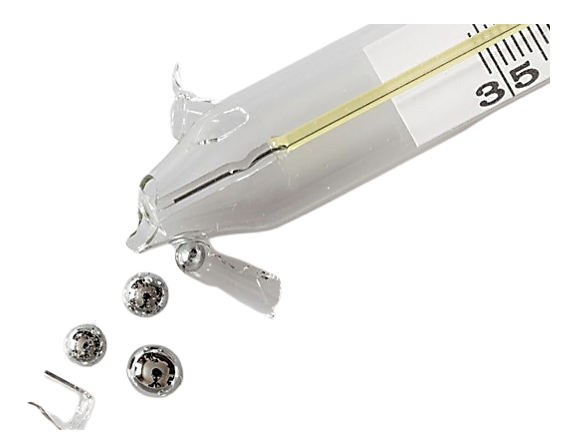
\includegraphics[scale=0.5]{figs/G10Y25B1-9}}
	\loigiai{Cách xử lí đúng nguyên tắc an toàn: báo cho giáo viên tại phòng thí nghiệm, sơ tán các bạn học sinh ở khu vực gần đó, tắt quạt và đóng hết cửa sổ để tránh việc thủy ngân phát tán trong không khí. Người dọn dẹp phải sử dụng găng tay và khẩu trang để dọn sạch thủy ngân, tuyệt đối không được tiếp xúc trực tiếp với thủy ngân bằng tay.}
\end{ex}
\begin{ex}
		\immini{Giới hạn đo của ampe kế ở hình bên là bao nhiêu? Nếu sử dụng ampe kế để đo dòng điện vượt quá giới hạn đo thì có thể gây ra nguy cơ gì?}
		{\vspace{-0.75cm}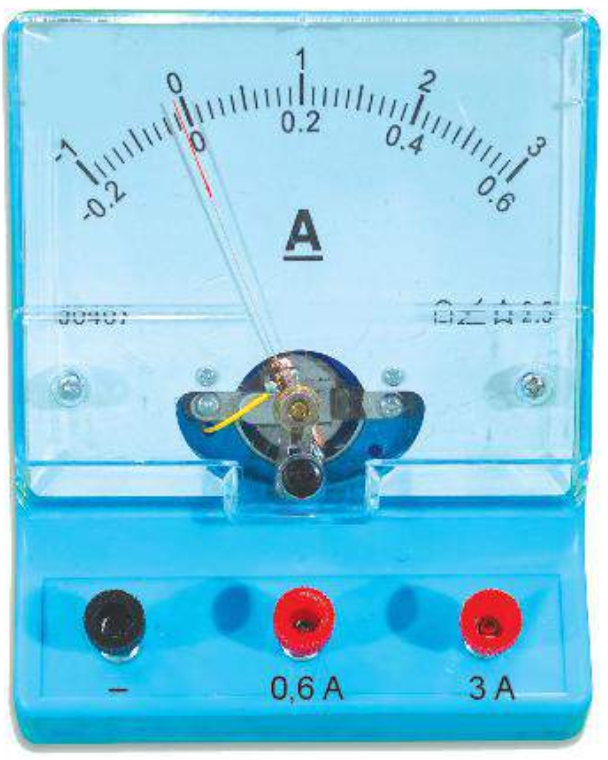
\includegraphics[scale=0.4]{figs/G10Y25B1-10}}
	\loigiai{
		Giới hạn đo là \SI{3}{A}.\\
		Nếu sử dụng ampe kế để đo dòng điện vượt quá giới hạn đo thì có thể làm cho ampe kế bị hư hỏng.
	}
\end{ex}
%\Closesolutionfile{ans}
>>>>>>> Stashed changes
